% Twenty values of prod_{p<=x}(1-1/p), coral, against e^{-gamma}/log x, charcoal.
% Abscissae: 10,15,20,30,50,75,100,150,200,300,500,750,1000,1500,2000,3000,5000,10000,20000,50000.
% log10(x) from 0.85 to 4.95 maps to width 5.8; values from 0.02 to 0.27 map to height 3.7.
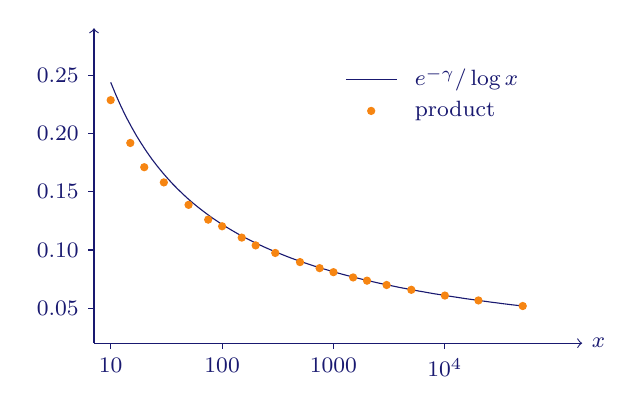
\begin{tikzpicture}[every node/.style={font=\footnotesize}]
\draw[MidnightBlue] (0.212,3.313) -- (0.278,3.153) -- (0.343,3.007) -- (0.408,2.873) -- (0.474,2.750) -- (0.539,2.635) -- (0.605,2.529) -- (0.670,2.430) -- (0.735,2.338) -- (0.801,2.252) -- (0.866,2.172) -- (0.932,2.096) -- (0.997,2.025) -- (1.063,1.958) -- (1.128,1.895) -- (1.193,1.835) -- (1.259,1.778) -- (1.324,1.725) -- (1.390,1.674) -- (1.455,1.625) -- (1.520,1.579) -- (1.586,1.535) -- (1.651,1.493) -- (1.717,1.453) -- (1.782,1.415) -- (1.847,1.378) -- (1.913,1.343) -- (1.978,1.309) -- (2.044,1.277) -- (2.109,1.246) -- (2.174,1.216) -- (2.240,1.187) -- (2.305,1.159) -- (2.371,1.133) -- (2.436,1.107) -- (2.501,1.082) -- (2.567,1.058) -- (2.632,1.035) -- (2.698,1.013) -- (2.763,0.991) -- (2.829,0.970) -- (2.894,0.950) -- (2.959,0.931) -- (3.025,0.912) -- (3.090,0.893) -- (3.156,0.875) -- (3.221,0.858) -- (3.286,0.841) -- (3.352,0.825) -- (3.417,0.809) -- (3.483,0.794) -- (3.548,0.779) -- (3.613,0.764) -- (3.679,0.750) -- (3.744,0.736) -- (3.810,0.723) -- (3.875,0.709) -- (3.940,0.697) -- (4.006,0.684) -- (4.071,0.672) -- (4.137,0.660) -- (4.202,0.649) -- (4.268,0.637) -- (4.333,0.626) -- (4.398,0.616) -- (4.464,0.605) -- (4.529,0.595) -- (4.595,0.585) -- (4.660,0.575) -- (4.725,0.565) -- (4.791,0.556) -- (4.856,0.547) -- (4.922,0.538) -- (4.987,0.529) -- (5.052,0.520) -- (5.118,0.512) -- (5.183,0.503) -- (5.249,0.495) -- (5.314,0.487) -- (5.379,0.480) -- (5.445,0.472);
\fill[BurntOrange] (0.212,3.087) circle[radius=1.5pt];
\fill[BurntOrange] (0.461,2.543) circle[radius=1.5pt];
\fill[BurntOrange] (0.638,2.235) circle[radius=1.5pt];
\fill[BurntOrange] (0.887,2.042) circle[radius=1.5pt];
\fill[BurntOrange] (1.201,1.757) circle[radius=1.5pt];
\fill[BurntOrange] (1.450,1.569) circle[radius=1.5pt];
\fill[BurntOrange] (1.627,1.485) circle[radius=1.5pt];
\fill[BurntOrange] (1.876,1.341) circle[radius=1.5pt];
\fill[BurntOrange] (2.053,1.242) circle[radius=1.5pt];
\fill[BurntOrange] (2.302,1.146) circle[radius=1.5pt];
\fill[BurntOrange] (2.616,1.030) circle[radius=1.5pt];
\fill[BurntOrange] (2.865,0.953) circle[radius=1.5pt];
\fill[BurntOrange] (3.041,0.902) circle[radius=1.5pt];
\fill[BurntOrange] (3.291,0.835) circle[radius=1.5pt];
\fill[BurntOrange] (3.467,0.794) circle[radius=1.5pt];
\fill[BurntOrange] (3.716,0.739) circle[radius=1.5pt];
\fill[BurntOrange] (4.030,0.678) circle[radius=1.5pt];
\fill[BurntOrange] (4.456,0.605) circle[radius=1.5pt];
\fill[BurntOrange] (4.882,0.543) circle[radius=1.5pt];
\fill[BurntOrange] (5.445,0.472) circle[radius=1.5pt];
\draw[MidnightBlue,->] (0,0)--(6.20,0);
\draw[MidnightBlue,->] (0,0)--(0,4.00);
\node[MidnightBlue,right] at (6.20,0) {$x$};
\draw[MidnightBlue] (0.212,0)--(0.212,-0.07) node[below] {$10$};
\draw[MidnightBlue] (1.627,0)--(1.627,-0.07) node[below] {$100$};
\draw[MidnightBlue] (3.041,0)--(3.041,-0.07) node[below] {$1000$};
\draw[MidnightBlue] (4.456,0)--(4.456,-0.07) node[below] {$10^{4}$};
\draw[MidnightBlue] (0,0.444)--(-0.07,0.444) node[left] {$0.05$};
\draw[MidnightBlue] (0,1.184)--(-0.07,1.184) node[left] {$0.10$};
\draw[MidnightBlue] (0,1.924)--(-0.07,1.924) node[left] {$0.15$};
\draw[MidnightBlue] (0,2.664)--(-0.07,2.664) node[left] {$0.20$};
\draw[MidnightBlue] (0,3.404)--(-0.07,3.404) node[left] {$0.25$};
\draw[MidnightBlue] (3.20,3.35)--(3.85,3.35);
\node[MidnightBlue,anchor=west] at (3.95,3.35) {$e^{-\gamma}/\log x$};
\fill[BurntOrange] (3.52,2.95) circle[radius=1.5pt];
\node[MidnightBlue,anchor=west] at (3.95,2.95) {product};
\end{tikzpicture}
